\begin{document}
	
	\subsection{Training}
	
	This step consist in the estimation of the centroids of the color space. May be  really time consuming, but it is performed only once. 
	To achieved the estimation of centroids, a k-means clustering of the multichannel images of several CT scan from different patients is performed. 
	In order to achieve a uniform representation of each cluster, the scans included in the training set were carefully selected from the $3$ datasets used in this work. The main rule used for the selection is that in each scan must be present a huge amount of infection areas and also a well representation of artifacts, in order to takes into account all the possible features.
	The achievement of the training task involves two main steps : 
	\begin{enumerate}
		\item \textbf{Preparation of images} : involves the building of the multi channel images, and the registration in a common space; 
		
		\item \textbf{Clustering} :% Actual clustering, involves also the managing of the background problem.
	\end{enumerate}

		\subsubsection*{Preparation of Images} 
		
		
	
		This step involves the preparation of images, with the building of the multi channel image that incorporates neighbouring and edges information as well as the registration in a common space and the managing of an allocation memory problem.\\
			
		The used image is composed by 4 channel built as follows:  
		\begin{itemize}
			\item Pure image after Contrast Limited Adaptive Histogram Equalization (CLAHE),whti a block sizeof  $10\times 10$ pixels
			\item Image after a median blurring with kernel size equal to $11$ pixes
			\item Image after a gamma correction with $\gamma = 1.5$
			\item Standard filtered image with a kernel of size $3$ pixels
		\end{itemize}
	
		\begin{figure}[h]
			\centering
				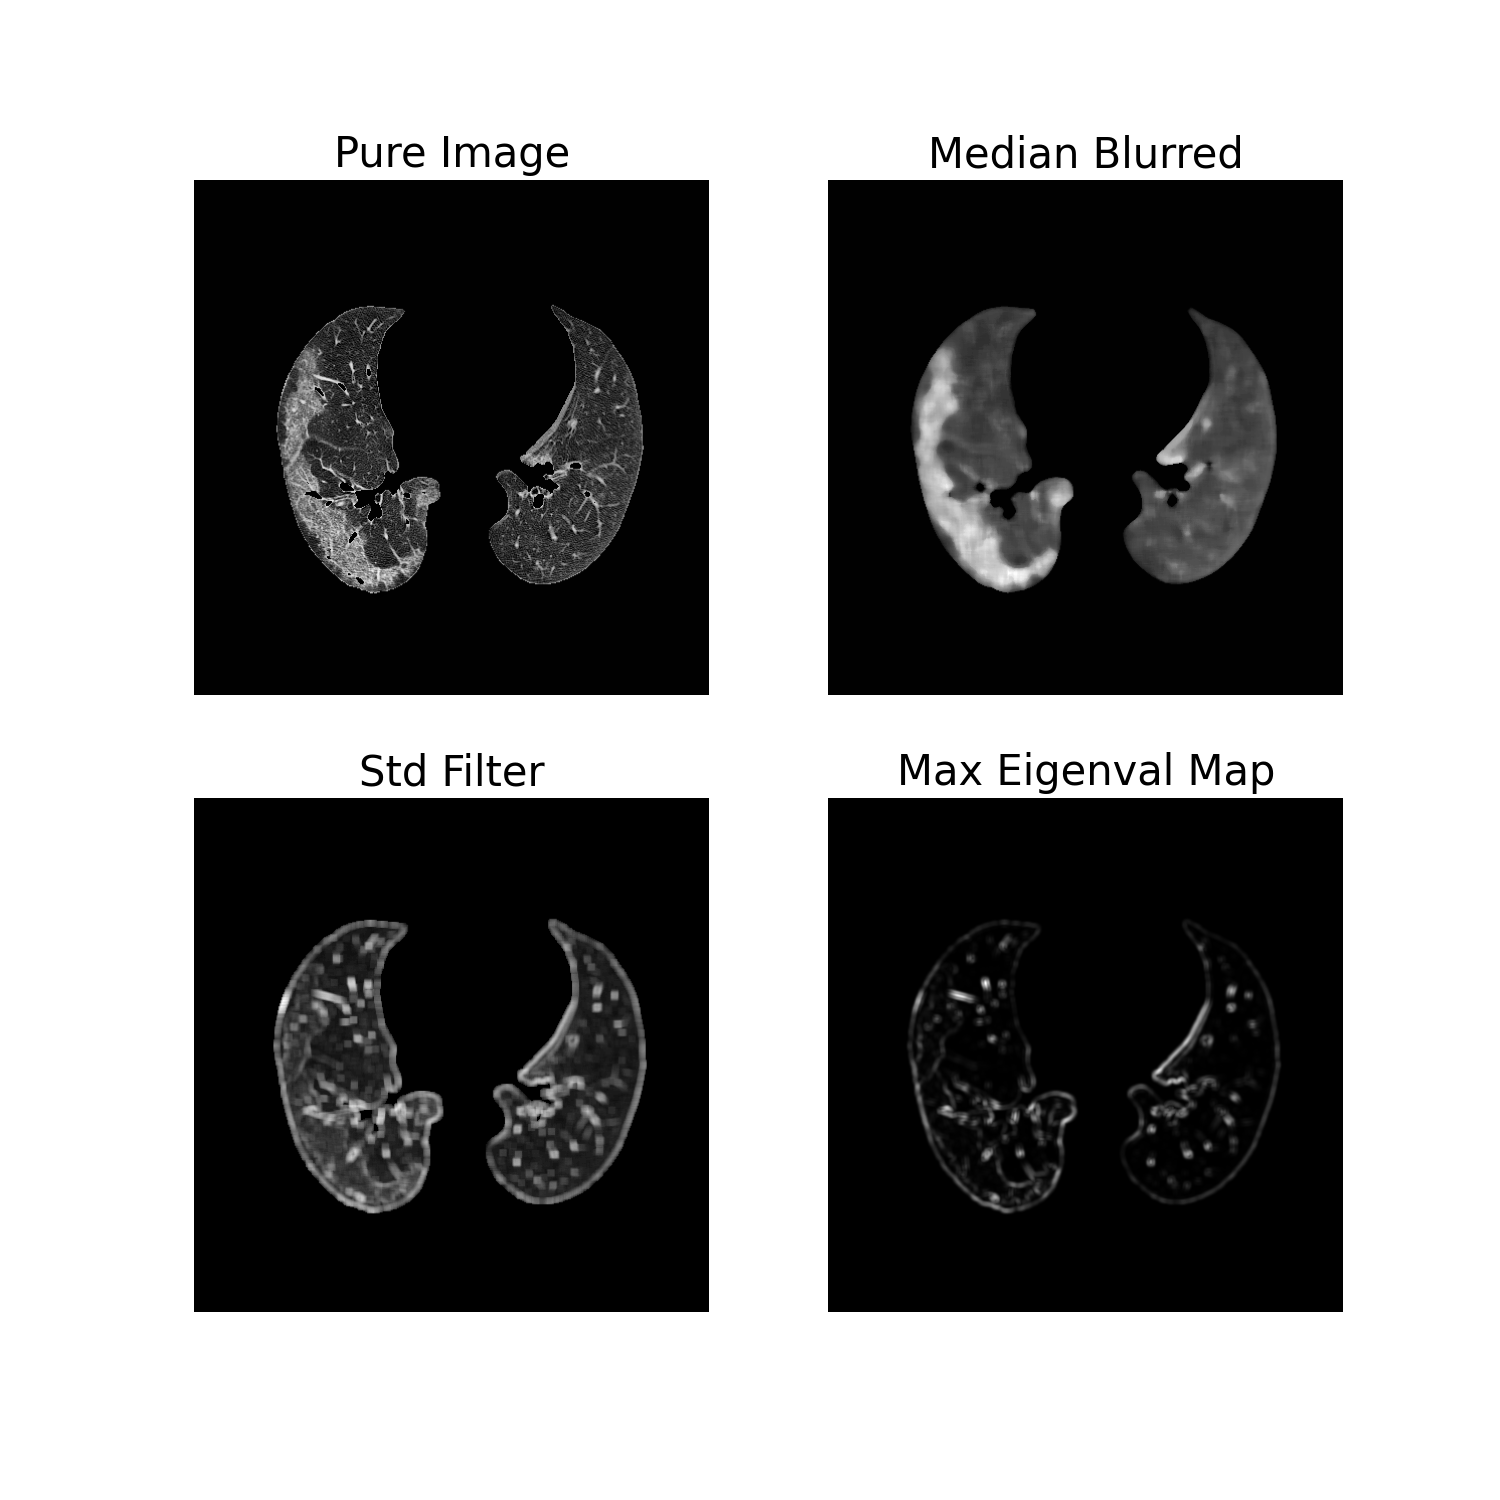
\includegraphics[scale=.55]{Multi_Channel.png}
			\caption{Channels of the image. From left to right and from top to bottom the image after the histogram equalization, the gamma correction, the median blurring and the std filtering. These channels allow us to consider information about single voxels, neighbouring voxels and their variability. The histogram eqaulization is applied over small $10\times 10$ areas to avoid  over-amplification of the contrast. The gamma correction was performed using $\gamma = 1.5$, and the median and std filter kernel sizes are respectively $11$ and $3$. Each image is normalized according to mean and standard deviation of the whole scan. }\label{fig:MultiChannel}
		\end{figure}
	
		In order to compute the different image filter, I've vectorize the corresponding \textsc{OpenCV} functions by iteration over the axial direction. Since these function requires as input an $8-$bit gray scale image, I've to rescale the input tensor.
	
		In \figurename\,\ref{fig:MultiChannel} I have displayed the 4 different channels of the image. Each channel allow us to consider different information.
		
		The histogram equalized image and the gamma corrected allows to take into account information about the single voxel. The histogram equalization is applied in order to enhance the image contrast by improving the GL usage. For each slice the histogram is equalized considering only a $10\times 10$ area, in order to take care of the over-amplification of the contrast.
		
		The gamma correction is a non linear operation and is used to decode the luminance, and to made in evidence the less evident lesions. Both of these filters involves the single voxel.
		
		The median blurring allow us to consider also the information of the neighborhood voxels, allowing the reduction of the outliers. The usage of the filter is justified since the lesions involves several closest voxels.
		 
		The last channel used is the image after the application of a local standard deviation filter which consist in the replacement of each pixel value with the standard deviation of its neighborhood, help us to distinguish the bronchial structures and motion artifacts not removed in the previous step.	
		Each image channel is normalized according to means and standard deviation of the whole scan.
		
		
		\subsubsection*{Clustering} 
		
		After the construction of the multichannel image of for each input series, all the images are shuffled and divided into several sub-samples. 
		
		The clustering was performed independently on each sub-sample and only the centroids set which minimize the intra cluster variance is taken. That because since the results of the k-means clustering depends on the initial choice centroids. Even if the k-means++ allows an optimal way to chose the initial centroids, also may happen that during the minimization of the potential function the algorithm found a local minimum rather than the global one. The different clustering allow us to estimate more than one possible solution and estimate chose the best one. 		
		Moreover the creation of several sub-samples is made since the creation of a single, huge array with several images is not always possible, since requires a huge quantity of memory to be allocated, so we have chose to divide all the images into several sub-samples and chose the optimal ones.
		
		As I have said before, the k-means clustering requires a balance in the different cluster representation. The problem of the under-represented clusters is overcome by a proper choose of the training set. To manage the over-represented cluster ( the background) and the clustering of the multiple subsamples, I have defined the \textsc{kmeans\_on\_subsamples} function. Implemented as follows.
		
		\lstset{style=python}
		\begin{lstlisting}[language=python, caption=kmenas\_on\_subsamples, label=code:kmeans]
			
		import cv2
		import numpy as np
		from tqdm import tqdm
			
		def kmeans_on_subsamples(imgs,  n_centroids, stopping_criteria, 
									centr_init, weight = None) :
			
			if weight is not None :
				vector = np.asarray([ el[w != 0] 
											for el, w in zip(imgs, weight)], dtype = np.ndarray)
			else :
			vector = np.asarray([el.reshape((-1, el[-1])) 
											for el in imgs], dtype=np.ndarray)
			
			centroids = []
			for el in tqdm(vector) :
			
				_, _, centr = cv2.kmeans(el.astype(np.float32), n_centroids, None, stopping_criteria, 10, centr_init)				
				centroids.append(centr)
			
			return np.asarray(centroids, dtype= np.float32)
			
		\end{lstlisting}
	
		As we can see the clustering of the different subsamples is managed simply iterating over the subsamples vector and storing the partial results in a list. The background removal is managed by passing a weight tensor. The value of this tensor must be zero for the voxel representing the background, and one otherwise. This allows to build the sample vector removing the background values.
			
		An other problem may be the estimation of the correct number of clusters since k-means clustering requires a prior knowledge on the number of clusters. In our case the anatomical knowledge about the lung may help, since we can consider one cluster for each anatomical structure. I have found that 5 clusters are a viable choice, and the considered structures are the following: 
		\begin{itemize}
		
			\item Lung Parenchima;
		
			\item Edges;
		
			\item Vessel surrounding bronchial structures;
			
			\item Ground Glass Opacities and consolidation;
		
			\item Bronchi.

		\end{itemize}

	
	The whole step is summarized in the pseudocode in \figurename\,\ref{alg:training}.
		
		
	\begin{algorithm}
	
	\SetAlgoLined
	\DontPrintSemicolon
	
	\KwData{CT scans with Extracted lung}
	\KwResult{Centroid matrix}\;
	
	\ForEach{$scan \in input\_scans$}{
	
		read the scan\;
		sample$\leftarrow$image\_array\;
	}\;
	\tcc{prepare subsamples}
	sample$\leftarrow$ build\_multichannel(sample)\;
	sample$\leftarrow$shuffle(sample)\;
	subsamples$\leftarrow$split(sample)\;
	
	\tcc{start the first clustering}
	\ForEach{$ Sub \in subsamples $}
	{
		center$\leftarrow$kmeans(sub, number of centroids)\;
		centroid\_vector, internal\_variance$\leftarrow$append(center)
		
	}\;

	\tcc{Refinement}
	centroid\_matrix$\leftarrow$centroid\_vactor($\min(internal\_variance$))\;
	
	\caption{Pseudo-code for the training script}\label{alg:training}
	
\end{algorithm}

	
\end{document}